\documentclass{ximera}
\graphicspath{
{./}
{volumes/}
{arclengths/}
{centroids/}
{techniques/}
{applications/}
{series/}
{powerseries/}
{odes/}
{lessons/}
}
\usepackage{booktabs}

\newcommand{\bigmath}[1]{$\displaystyle #1$}
\newcommand{\choicebreak}{}
\newenvironment{type}{}{}
\newenvironment{notes}{}{}
\newenvironment{keywords}{}{}
\newcommand{\offline}{}
\newenvironment{comments}{\begin{feedback}}{\end{feedback}}
\newenvironment{multiplechoice}{\begin{multipleChoice}}{\end{multipleChoice}}
\title{The Disk and Washer Methods}
\author{Philip T. Gressman}

\begin{document}
\begin{abstract}
  We practice setting up calculations related to the disk and washer methods.
\end{abstract}
\maketitle

\begin{example}
Suppose the region below the graph $y = \sqrt{\sin x}$ and above the $x$-axis between $x=0$ and $x=\pi$ is revolved around the $x$-axis. Compute the volume of the resulting solid.
\begin{center}
\begin{image}
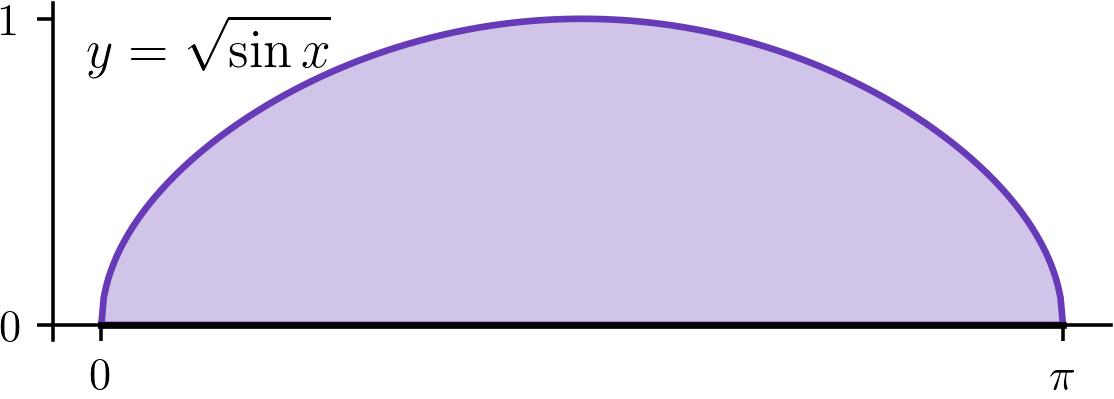
\includegraphics[width=4in]{diskwasher/disksin.png}
\end{image}
\end{center}
\begin{itemize}
\item Because the axis of rotation lies perfectly along the boundary of the region, the \wordChoice{\choice[correct]{disk}\choice{washer}} method can be used.
\item The radius $R$ is the length of a \wordChoice{\choice{horizontal}\choice[correct]{vertical}} extending from the axis to the graph $y = \sqrt{\sin x}$.
\item Thus we know that the radius $R$ must equal
\begin{multipleChoice}\choice[correct]{$R(x) = \sqrt{\sin x} - 0 = \sqrt{\sin x}$}\choice{$R(y) = \arcsin y^2 - 0 = \arcsin y^2$}\end{multipleChoice}
\item We conclude that
\[ V = \int_{\answer{0}}^{\answer{\pi}} \pi \left( \answer{\sqrt{\sin x}} \right)^2 d\answer{x} = \answer{2\pi}. \]
\end{itemize}
\end{example}

\begin{example}
Suppose the region between the graphs $y = x/2$ and $y=x^2/4$ is revolved around the axis $x=0$. Compute the volume of the resulting solid.
\begin{center}
\begin{image}
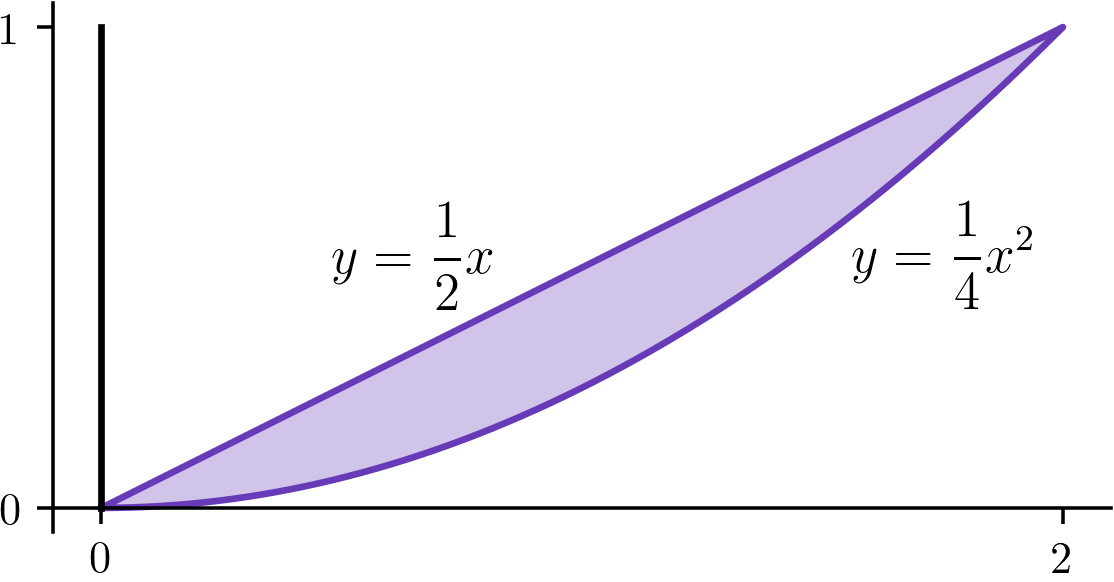
\includegraphics[width=4in]{diskwasher/washer1.png}
\end{image}
\end{center}
\begin{itemize}
\item Because the axis of rotation does not lie along the boundary of the region, the \wordChoice{\choice{disk}\choice[correct]{washer}} method can be used.
\item In this case, radius will equal the length of a \wordChoice{\choice[correct]{horizontal}\choice{vertical}} extending from the axis to the graphs $y = x/2$ and $y = x^2/4$.
\item 
\begin{multipleChoice}
\choice{$R_{\mathrm{outer}} (x) = x/2 $ and $r_{\mathrm{inner}}(x) = x^2/4$}
\choice[correct]{$R_{\mathrm{outer}} (y) = 2 \sqrt{y} $ and $r_{\mathrm{inner}}(y) = 2 y$}
\end{multipleChoice}
\item We conclude that
\[ V = \int_{\answer{0}}^{\answer{1}} \pi \left[  \left( \answer{2 \sqrt{y}} \right)^2 - \left( \answer{2 y} \right)^2  \right] d\answer{y} = \answer{\frac{2 \pi}{3}}. \]
\end{itemize}
\end{example}


\end{document}
